% Made up for the tikra gallery: a rose r = cos(k theta); an odd k gives k petals, an even k twice as many.
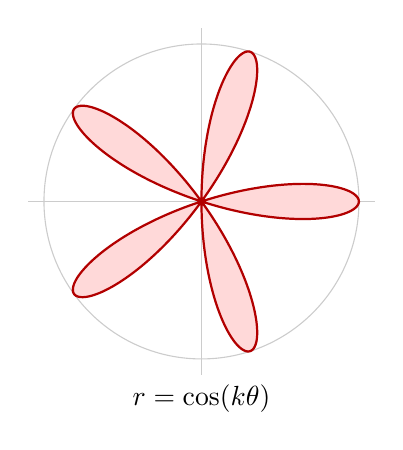
\begin{tikzpicture}
  \def\k{5}   % the petals, 1..9
  \draw[gray!40] (0,0) circle (2);
  \draw[gray!40] (-2.2,0) -- (2.2,0) (0,-2.2) -- (0,2.2);
  \filldraw[red!70!black, fill=red!15, thick, domain=0:360, samples=400, smooth] plot (\x:{2*cos(\k*\x)}) -- cycle;
  \node[below] at (0,-2.2) {$r = \cos(k\theta)$};
\end{tikzpicture}
